\chapter{Аналитический раздел}

В данном разделе будут формализованы объекты сцены, выбран способ заданий моделей, алгоритм удаления невидимых линий и поверхностей и алгоритм закраски.

\section{Формализация объектов синтезируемой сцены}

Сцена состоит из следующих объектов:
\begin{itemize}[label=---]
	\item \textbf{Камера} -- специальный объект сцены, позволяющий просматривать ее сцены. Камера определяется двумя точками пространства: местоположением самой камеры, и точкой, к которой направлен объектив камеры;
	
	\item \textbf{Источник света} -- объект сцены, который представляет из себя материальную точку, излучающую свет во всех направлениях. Источник света отображается как несколько концентрических окружностей;
	
	\item \textbf{Модель} -- трехмерный объект, расположенный на сцене.
\end{itemize}

\section{Анализ типов трехмерных моделей}

Тип трехмерной модели определяет, как именно объект будет отображаться на сцене.

Модели могут задаваться в следующих формах:

\begin{itemize}[label=---]
	\item \textbf{Каркасная модель.} Это простейшая форма задания модели. Каркасная модель хранит информацию о вершинах и ребрах объекта. Основной недостаток такого отображения объектов заключается в том, что модель не всегда однозначно передает представление о форме объекта, в следствии чего ее можно неправильно интерпретировать.
	\item \textbf{Поверхностная модель.} Этот тип модели хранит информацию о каждой поверхности объекта. Поверхность может описываться аналитически, либо задаваться другим способом. Одним из недостатков поверхностной модели является отсутствие информации о том, с какой стороны поверхности находится материал.
	\item \textbf{Твердотельная модель.} Данный тип задания модели отличается от поверхностного тем, что в твердотельных моделях к информации о поверхностях добавляется информация о том, с какой стороны расположен материал. Это можно сделать, например, путем указания направления внутренней нормали. 
\end{itemize}

\subsection*{Вывод}
Использовать каркасный тип модели в моей задачи нецелесообразно, потому что такой тип в некоторых случаях может запутать пользователя, не давая полного представления об объекте.

Использовать твердотельную модель просто нет необходимости, т.к. пользователю моей программы не важно, с какой стороны от модели находится материал.

Поэтому я принял решение использовать полигональный тип модели, как самый подходящий для моей задачи. Тем не менее, моя программа предоставляет возможность отображения модели и в каркасной форме.


\section{Анализ способов задания поверхностной модели}

Поверхностную модель можно задать несколькими способами:
\begin{itemize}[label=---]
	\item \textbf{Аналитический способ.} Этот способ задания модели характеризуется описанием модели объекта, которое доступно в неявной форме. То есть для получения визуальных характеристик необходимо дополнительно вычислять некоторую функцию, которая зависит от параметра.
	\item \textbf{Полигональная сетка.} Данный способ позволяет задать модель совокупностью вершин, ребер и граней, определяющих ее форму в трехмерном пространстве.
\end{itemize}

Рассмотрим существующие способы хранения информации о полигональной сетке.

\begin{itemize}[label=---]
	\item \textbf{Вершинное представление.} Модель хранит множество вершин. Вершины указывают на другие вершины, с которыми они соединены.
	\item \textbf{Список граней.} Модель хранит множество граней и множество вершин. Каждая вершина при этом хранит информацию о соседних вершинах и о гранях, ее окружающих.
 	\item \textbf{Крылатое представление.} Модель хранит информацию о вершинах, ребрах и гранях. При этом каждая вершина и грань хранят окружающие их ребра, а каждое ребро состоит из двух вершин (конечные точки), двух граней (по каждую сторону), и четырех ребер (<<крылья>> ребра).
	\item \textbf{Таблица углов.} Модель задается таблицей, хранящей вершины. Обход заданной таблицы неявно задает полигоны.
\end{itemize}

\subsection*{Вывод}

Использовать для моей задачи аналитический способ невозможно, так как задача предполагает возможность изменение модели посредством трансформации ее составляющих элементов.

Выбор конкретного способа хранения сетки напрямую зависит от поставленной задачи. Моя программа должна предоставлять возможность быстрого выбора и трансформации любых вершин, ребер и граней. Соответственно, решающим фактором является скорость выполнения этих операций. Поэтому полигональная сетка должна явно хранить информацию о каждой этой составляющей объекта. 

Все вышеописанные способы, помимо крылатого представления, не хранят в явном виде информацию о ребрах, хотя в моей программе эта информация необходима. Крылатое представление же избыточно для моей задачи. 

Поэтому я разработал собственный способ хранения информации о сетке. В качестве основы был взят список граней, к которому я добавил информацию о ребрах, которые определяются двумя конечными точками. Иными словами, модель должна состоять из следующих элементов:
\begin{enumerate}
	\item \textbf{Вершина.} Задается начальными координатами в пространстве и матрицей трансформации.
	
	\item \textbf{Ребро.} Задается двумя его конечными вершинами.
	
	\item \textbf{Грань.} Задается набором принадлежащих ей вершин и ребер.
	
\end{enumerate}

Сама модель определяется набором принадлежащих ей граней, ребер и вершин.

\section{Анализ способа выбора элементов модели на дисплее}

Специфика моей задачи предполагает, что программа должна предоставлять пользователю возможность выбора необходимых ему вершин, ребер и граней при помощи клика мышью по дисплею вблизи них. Более того, пользователь должен иметь возможность выбрать только те элементы фигуры, которые являются видимыми. 

Для решения этой проблемы было принято решение помимо буфера кадра хранить еще и буфер граней, каждая ячейка которого будет указывать на грань, которая отображается в соответствующей ячейке буфера кадров. Буфер граней позволит за константное время определить, какую именно грань выбрал пользователь и найти ближайшие к месту клика мыши вершину или ребро.

\section{Анализ алгоритмов удаления невидимых линий и поверхностей}

При выборе алгоритма удаления невидимых линий необходимо в первую очередь учесть особенности поставленной задачи. Моя задача подразумевает, что алгоритм удаления невидимых линий будет быстродействующим, поскольку пользователь должен видеть плавную анимацию при трансформации моделей или камеры. Также немаловажное значение имеет сложность реализации определенного алгоритма. Кроме того, выбранный алгоритм должен позволять быстро и эффективно заполнять буфер граней, описанный в предыдущем пункте.

При этом не имеет значения, в каком пространстве работает алгоритм, так как для моей задачи скорость важнее точности.

\subsection{Алгоритм Робертса}

Алгоритм Робертса \cite{rogers_alg} --- алгоритм удаления невидимых граней и поверхностей, работающий в объектном пространстве, решая задачу только с выпуклыми телами.

Алгоритм выполняется в 3 этапа.
\begin{enumerate}[]
	\item \textbf{Этап подготовки исходных данных.} 	На данном этапе должна быть задана информация о телах. Для каждого тела сцены должна быть сформирована матрица тела V. Размерность матрицы – $4 \cdot n$, где $n$ – количество граней тела. Каждый столбец матрицы представляет собой четыре коэффициента уравнения плоскости $ax+by+cz+d=0$, проходящей через очередную грань. 
	
	Матрица тела должна быть сформирована корректно, то есть любая точка, расположенная внутри тела, должна располагаться по положительную сторону от каждой грани тела. В случае, если для очередной грани условие не выполняется, соответствующий столбец матрицы надо умножить на -1. Для проведения проверки следует взять точку, расположенную внутри тела.
	
	\item \textbf{Этап удаления ребер, экранируемых самим телом.} На данном этапе рассматривается вектор взгляда E = \{0, 0,-1, 0\}. Для определения невидимых граней достаточно умножить вектор E на матрицу тела V. Отрицательные компоненты полученного вектора будут соответствовать невидимым граням.
	
	\item \textbf{Этап удаления невидимых ребер, экранируемых другими телами сцены.} На данном этапе для определения невидимых точек ребра требуется построить луч, соединяющий точку наблюдения с точкой на ребре. Точка будет невидимой, если луч на своем пути встречает в качестве преграды рассматриваемое тело. Если тело является преградой, то луч должен пройти через тело. Если луч проходит через тело, то он находится по положительную сторону от каждой грани тела.	
\end{enumerate}

Основным преимуществом данного алгоритма является точность вычислений. Она достигается за счет работы в объектном пространстве, в отличии от большинства других алгоритмов.
 
Серьезным недостатком является вычислительная трудоемкость алгоритма. В теории она растет как квадрат количества объектов. Поэтому при большом количестве объектов на сцене, этот алгоритм будет работать достаточно медленно. Но для решения этой проблемы можно использовать разные оптимизации для повышения эффективности, например, сортировку по оси z. Тем не менее, некоторые из оптимизаций крайне сложны, что затрудняет реализацию этого алгоритма.

Еще один весомый недостаток этого алгоритма - все тела сцены должны быть выпуклыми. Данная проблема также приводит к усложнению алгоритма, так как потребуется прибегнуть к проверке объектов на выпуклость и их разбиению на выпуклые многоугольники, что сильно замедлит алгоритм при большом количестве тел.

\clearpage

\subsubsection*{Вывод}

Алгоритм Робертса не подходит для решения поставленной задачи по следующим причинам:

\begin{itemize}[label=---]
	\item от программы не требуется той точности визуализации объектов, которую предоставляет этот алгоритм;
	\item на сцене может находиться множество объектов (зачастую - невыпуклых), что сильно замедлит скорость работы алгоритма. Таким образом, алгоритм не удовлетворяет требованиям к скорости выполнения алгоритма;
	\item реализация модификаций, позволяющих приблизить рост сложности алгоритма к линейной, очень трудозатратна;
	\item при использовании этого алгоритма возникают трудности с заполнением <<буфера граней>>.
\end{itemize}

\subsection{Алгоритм Варнока}

Алгоритм Варнока \cite{rogers_alg} --- алгоритм удаления невидимых граней и поверхностей, работающий в пространстве изображения.

Основной идеей данного алгоритма является рекурсивное разбиении области экрана на более мелкие подобласти (рисунок \ref{fig:varnok}). Для каждой подобласти определяются связанные с ней многоугольники и те из них, видимость которых тривиальна, изображаются на экране. В случае невозможности однозначно определить видимость части многоугольника разбиение области повторяется, и для каждой из вновь полученных подобластей рекурсивно применяется процедура определения видимости. В результате работы алгоритма получаются области, содержащие не более одного многоугольника, либо разбиение продолжается до тех пор, пока размер области не станет равен одному пикселю. В этом случае для полученного пикселя вычисляется значение глубины каждого многоугольника (координата Z), и визуализируется тот из них, у которого значение этой координаты больше.

\begin{figure}[h]
	\centering
	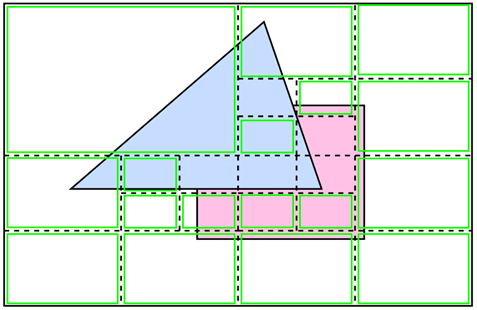
\includegraphics[scale=1]{inc/img/Varnok.png}
	\caption{Разбиении области экрана алгоритмом Варнока}
	\label{fig:varnok}
\end{figure} 

Достоинством данного алгоритма является простота реализации и высокая эффективность в случае, если размеры перекрываемых областей невелики.

Его главным недостатком является использование рекурсивных вызовов, что значительно снижает скорость выполнения в случае больших размеров перекрываемых областей.

\subsubsection*{Вывод}

Алгоритм Варнока не подходит для решения моей задачи по следующим причинам:

\begin{itemize}[label=---]
	\item алгоритм зависит от количества перекрывающихся областей на сцене, поэтому при его использовании отрисовка сцены может работать неоднородно;
	\item при использовании этого алгоритма возникают трудности с заполнением <<буфера граней>>.
\end{itemize}

\subsection{Алгоритм, использующий Z-буфер}

Алгоритм, использующий Z-буфер \cite{rogers_alg} --- алгоритм удаления невидимых граней и поверхностей, работающий в пространстве изображения.

Идея алгоритма, использующего Z-буфер (далее -- алгоритм Z-буфера) заключается в использовании буфера, хранящего глубину каждого пикселя.

В ходе работы алгоритма значение глубины каждого нового пикселя, заносимого в буфер кадра, сравнивается с глубиной того пикселя, который уже занесен в Z-буфер. Если это сравнение показывает, что новый пиксель расположен ближе к наблюдателю, чем пиксель, уже находящийся в буфере кадра, то новый пиксель заносится в буфер кадра и производится корректировка Z-буфера: в него заносится глубина нового пикселя. Если же значение глубины нового пикселя меньше, чем хранящееся в буфере, то осуществляется переход к следующей точке.

Достоинством данного алгоритма является его простота, которая не мешает решению задачи удаления поверхностей и визуализации их пересечения. Также в этом алгоритме отсутствует необходимость предварительной сортировки объектов по глубине, то есть они могут обрабатываться в произвольном порядке. Более того, время работы алгоритм линейно зависит от количества граней на сцене, что делает его одним из самых быстродействующих. Помимо прочего, важным преимуществом этого алгоритма является возможность применения параллельных вычислений.

Недостаткам данного алгоритма является необходимость выделения памяти под два буфера, каждый из которых имеет размер равный количеству пикселей на экране, но для современных компьютеров этот недостаток является незначительным.

\subsubsection*{Вывод}

Данный алгоритм наилучшим образом подходит для решения поставленной задачи, так как:

\begin{itemize}[label=---]
	\item из-за отсутствия необходимости предварительной сортировки, алгоритм способен работать быстрее других даже с множеством объектов на сцене;
	\item при использовании этого алгоритма можно реализовать заполнение <<буфера граней>> вместе с заполнением двух других буферов;
	\item при реализации этого алгоритма возможно использование многопоточности.
\end{itemize}

\subsection{Алгоритм обратной трассировки лучей}

Алгоритм обратной трассировки лучей \cite{rogers_alg} --- алгоритм удаления невидимых граней и поверхностей, работающий в пространстве изображения.

Идея данного алгоритма заключается в том, что для каждого пикселя картинной плоскости определяется ближайшая к нему грань. Для этого через пиксель выпускается луч, находятся все пересечения луча с гранями и среди пересечений выбирается ближайшее.

К достоинствам данного алгоритма можно отнести возможность получения изображения гладких объектов без аппроксимации их примитивами (например, треугольниками). Благодаря отслеживанию пути, пройденного лучом, появляется возможность реализовать глобальную модель освещения, учитывающую отражения и преломления света. Качество полученного изображения получается очень реалистичным, этот метод отлично подходит для создания фотореалистичных сцен. Также важным преимуществом этого алгоритма является возможность применения параллельных вычислений, т.к. расчет отдельной точки выполняется независимо от других точек.

Главным недостатком алгоритма трассировки является необходимость создавать большое число лучей, проходящих через сцену, которые могут раздваиваться на отраженный и преломленный лучи, для которых все вычисления повторяются. Это приводит к существенному снижению скорости работы программы.

\subsubsection*{Вывод}

Данный алгоритм не отвечает главному требованию – скорости работы. От реализуемого продукта не требуется высокой реалистичности синтезируемого изображения и возможности работы с поверхностями, заданными в математической форме. Также в моей программе не предполагается присутствие эффектов отражения и преломления света. Таким образом, при заметном замедлении работы программы, качество изображения заметно не улучшится. Указанные факты говорят о том, что использовать алгоритм обратной трассировки лучей для моей задачи нецелесообразно.

\subsection{Выбор оптимального алгоритма}
С учетом изложенных выше заключений, в качестве алгоритма удаления невидимых линий и поверхностей был выбран алгоритм, использующий Z-буфер.

\section{Анализ методов закраски граней}

Существуют три основных алгоритма, позволяющих закрасить полигональную модель: простая закраска, закраска по Гуро и закраска по Фонгу.

\subsection{Простая закраска}

Суть алгоритма простой закраски \cite{rogers_alg} заключается в том, что для каждой грани объекта находится вектор нормали, и с его помощью в соответствии с выбранной моделью освещения вычисляется значение интенсивности, с которой закрашивается вся грань.

Данный метод закраски обладает большим быстродействием, так как его сложность линейно зависит от количества граней на сцене, однако все пиксели грани имеют одинаковую интенсивность, и сцена выглядит нереалистично. Тем не менее, этот метод крайне прост в реализации и совершенно не требователен к ресурсам.

\begin{figure}[h]
	\centering
	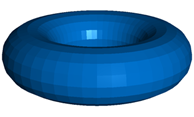
\includegraphics[scale=0.7]{inc/img/simple.png}
	\caption{Пример простой закраски}
	\label{fig:simple}
\end{figure} 

\subsection{Закраска по Гуро}

Основная идея алгоритма закраски по Гуро \cite{rogers_alg} заключается в билинейной интерполяции интенсивностей, за счет которой устраняется дискретность изменения интенсивности и создается иллюзия гладкой криволинейной поверхности. Иначе говоря, разные точки грани закрашиваются с разными значениями интенсивности.

С помощью этого метода получаются достаточно реалистичные изображения, однако все объекты кажутся матовыми.

\begin{figure}[h]
	\centering
	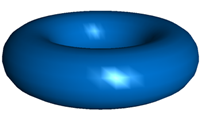
\includegraphics[scale=0.7]{inc/img/guro.png}
	\caption{Пример закраски по Гуро}
	\label{fig:guro}
\end{figure} 

\subsection{Закраска по Фонгу}

Закраска по Фонгу \cite{rogers_alg} по своей идее похожа на закраску по Гуро, но ее отличие состоит в том, что в методе Гуро по всем точкам полигона интерполируются значения интенсивностей, а в методе Фонга – вектора нормалей, и с их помощью для каждой точки находится значение интенсивности.

Эта закраска требует больших вычислительных затрат, чем предыдущие, однако она позволяет достигнуть лучшей локальной аппроксимации кривизны поверхности и, следовательно, с ее помощью получается более реалистичное изображение.

\begin{figure}[h]
	\centering
	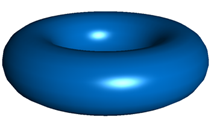
\includegraphics[scale=0.7]{inc/img/fong.png}
	\caption{Пример закраски по Фонгу}
	\label{fig:fong}
\end{figure} 


\subsection{Выбор оптимального алгоритма закраски}
Моя задача предполагает, что пользователь должен четко видеть ребра и вершины редактируемой модели. А закраски по Фонгу и Гуро будут сглаживать ребра, тем самым мешая пользователю сосредоточиться на моделировании. К тому же, они будут замедлять время отрисовки сцены.

Таким образом, для моей задачи оптимальным выбором будет простой алгоритм закраски.




